\documentclass[a4paper, 11pt, onecolumn]{article} 

% arara: pdflatex 
% arara: bibtex
% arara: pdflatex
% arara: pdflatex
% arara: clean: {extensions: [ aux, bbl, out, toc, blg, thm ]}

\input{Preamble}

%\usepackage{fonttable}

\usepackage{import}

\usepackage[
singlelinecheck=false % <-- important
]{caption}

\usepackage{upgreek}

\newcommand{\ie}{\textit{i.e.}}


% *****************************************************************
% Interlignes et marges
% *****************************************************************
\setstretch{1}
\geometry{%
left=2.5cm,
right=2.5cm,
top=2.5cm,
bottom=2.5cm,
%includefoot,
%headsep=1cm,
%footskip=1cm
}%

% *****************************************************************
% Page de garde
% *****************************************************************
\title{Indebtedness in Rural India: The Contribution of Cognitive Skills and Personality Traits}
\author{Arnaud Natal\thanks{Univ. Bordeaux, CNRS, GREThA, UMR 5113, F-33600 \textsc{Pessac, France} - \email{arnaud.natal@u-bordeaux.fr}} ~ \& Christophe J. Nordman\thanks{IRD, UMR LEDa-DIAL, IFP - \email{nordman@dial.prd}} }
\date{\today}
\renewcommand\maketitlehookc{%
  \begin{center}
    %\textsuperscript{1}{\small Université de Bordeaux}
    \textsuperscript{}{\normalsize Preliminary draft}
  \end{center}}

% ******************************************************************
\begin{document}
\maketitle

\hrule 
\vspace{0.3cm}

\begin{resab}{Abstract}

\end{resab}

\begin{motkey}{Keywords}
Gender, caste, 
\end{motkey}


\hrule
%\linenumbers

% ******************************
\section{Introduction}
%\addcontentsline{toc}{section}{Introduction}
\label{Introduction}
% ******************************
		% ******************************
		\subsubsection{Accroche}
		% ******************************
Despite the recent economic growth\footnote{Chiffre de la Banque Mondiale} and the improvement in education and health, social disparities subsist in India, especially through the caste system and gender.
Historically, caste --or \jati -- represent an hierarchical and endogamous group of individuals based on occupation.
With gender, it represent the major sources of inequality in terms of education \citep{Munshi2006, Hasan2006, Saha2013}, labour \citep{Madheswaran2007, Mohanty2006, Das2012}, wealth and poverty \citep{Borooah2005b, Zacharias2011, Deshpande2000, EsteveVolart2004} or marriage \citep{Banerjee2009, Chacko2003}.

		% ******************************
		\subsubsection{Conditioned individuals through caste and gender with aspirations}
		% ******************************
More recently, several works highlight disparities between \jati and gender in terms of aspirations.
\cite{Mukherjee2017} show that ``gender and caste primes can significantly affect long run aspirations and beliefs''. 
\cite{Alvi2019} use priming \footnote{} to study the effect of identity salience on aspirations.
They find that ``when women are primed on gender, they exhibit higher aspirations for their daughters [and] low-case  women primed on caste are more aspirational for their daughters''.
Finally, \cite{Sarkar2020} show that caste and gender work as double jeopardy instead of intersectionality for aspirations.
Indeed, ``the most socially disadvantaged groups -- Scheduled Tribe (ST) and Scheduled Caste (SC) -- have significantly lower income aspiration when compared to Other Backward Class (OBC) and Other Caste (OC) partiipants'' [and] [f]emale participants also have significantlty lower aspiration than their male counterparts''.
Moreover, SC/ST female participants have lower income aspiration levels compared to other groups.
Thus, beyond being a source of inequality, \jati and gender seems to deeply impact individuals by conditioning them.
More than an fregmentation and more than sources of dispartities, caste and gender seems to deeply impact social identities of individuals in India.
Indeed, it seems to conditionned individuals, it is part of their identity that affect action deep inside them as determine their aspirations.
In this context it appears important to analyse the role of personality traits \& cognitive skills on debt in take into account the deepness of this social identity.
For that, we use sub-sampling technic and we analyse the role of cognitive skills into this specific social identity.
We create four group of individual : female dalits (i); male dalits (ii); female middle and upper class (iii); male middle and upper class (iv). 
Three groups on four appears to be socially disadvantaged and one support the double jeopardy (DJ) thanks to \cite{Sarkar2020} (see Table \ref{tab:subsampling}).


Aspirations limitée par notre caste et notre sexe.



	% ******************************
	\subsection{Debt}
	% ******************************
	
Less work try to understand this disparities in terms of debt while it is an important research topic.
		
		% ******************************
		\subsubsection{Universality of debt with disparities which makes research interesting and important}
		% ******************************
\begin{itemize}
\item How much HH are concerned?
The Indian context is unique compared to other developping countries like China in terms of household finance.
Especially the role of retirement assets, gold and debt are unusual in the international context \citep{Badarinza2016b}.
To follows our research questions we only focuses\footnote{\cite{Badarinza2016b} developed the role of retirement assets and gold.} on debt.

\item Amount?
\item Sources?
The largest part of households debt is informal in rural India.
Compared to China, a tiny part of households have a mortgage loan --which is a classic formal loan \citep{Badarinza2016b}.

Constat: peu de formel, énormément d'informel
1. car les terres et les maisons s'héritent : \citep{Badarinza2016b} avancent que cela peut provenir de la « prédominance des ménages multigénérationnels, dans lesquels les terres et les propriétés résidentielles constituent une part importante des legs » donc pas beaucoup besoin d'emprunt formel. 4\% des ménages dont le chef a moins de 35 ans ont un prêt hypothécaire ce qui est nettement inférieur à la situation des autres pays émergents comme la Chine \citep{Badarinza2016b}.

2. Pénétration bancaire très hétérogène : \citep{Badarinza2016b} et \citep{Burgess2005} : les États ayant un taux de pénétration bancaire élevé sont ceux où les ménages sont les moins dépendants de l’endettement non institutionnel.

D'après \citep{Badarinza2016b}, la proba de contracter une dette informelle se réduit avec le niveau d'éducation: [l]es ménages dont au moins un membre a fait des études supérieures ou des études de troisième cycle ont une dette hypothécaire supérieure de 15,1\% par rapport au groupe des personnes peu instruites et une part de dette non institutionnelle inférieure de 28,7\%.

\item Reasons?

\item Determinants?  \citep{Datta2018, Pandey2016}

\item Failures for repayment, violence, overindebtedness, microcredit \citep{Sedai2021}
\item Disparities 
	\begin{itemize}
	\item \cite{Guerin2013} show that caste affect borrowing strategies as amount, type and source of debt in rural India.
	Moreover, they show that debt is a ``social transaction which inscribes debtors and creditors into local system of hierarchies''.
	\item \cite{Reboul2021} find an interest in the gender perspective.
	\item Debt bondage for dalits \citep{Guerin2020a}
	\item The case of microfinance for womens \citep{Guerin2020b}
	\item  Castes, sex, moc, etc.  \citep{Guerin2012a} \citep{Guerin2013a} \citep{Guerin2014} \citep{Reboul2020}
	\end{itemize}
\end{itemize}



		% ******************************
		\subsubsection{Importance of individual debt in terms of public policies}
		% ******************************

\begin{itemize}
\item Financial inclusion : more and more HH are financial included \citep{Badarinza2019}, especially in India \citep{Chakravartya2013}. \dev{Develop with Isabelle papers}
\item Secondly, on a vue que quasi tout le monde est concernés par la dette et especially to consume which is an determinants of global wealth\footnote{Expenditures approach of GDP.}.
In India, the households and non-profit institutions serving households (NPISHs) final consumption expenditure represent 60.29\% of GDP\footnote{World Bank Data - \url{https://data.worldbank.org/indicator/NE.CON.PRVT.ZS?locations=IN}. Accessed January 22, 2021.}.
\item Household finance has faced a renewed interest since a decade \citep{Guiso2013}.
Indeed, household are more implicated in financial decision such as privatization of retirement pension, liberalization of loan market, increase in credit purchase, which are more complicated because of financial innovation\footnote{For a comprehensive review on the subject, see \cite{Tufano2003}.}.
%Household finance (or consumer finance for researchers in business sciences) refer to the way that ``households use financial instruments to attain their objectives'' \citep{Campbell2006}.
%More precisely\footnote{For a comprehensive review on household finance, see \cite{Tufano2009} for whom household finance is ``the study of how institutions provide goods and services to satisfy the financial functions of households, how consumers make financial decisions, and how government action affects the provision of financial services'', \cite{Guiso2013}, or \cite{Xiao2020}.}  its a ``research field to study how financial institutions provide products and services to meet financial needs of consumers, how consumers make financial decisions, how government agencies regulate financial institutions and protect financial consumers and how science and technology help optimize the efficiency of consumer finance markets and improve social welfare'' \citep{Xiao2020}.
\end{itemize}





		% ******************************
		\subsubsection{Debt is not just money, it is social link}
		% ******************************
\begin{itemize}
\item Rapport de force
\item Prestige sociale
\end{itemize}

Dimension psychologique de la dette très importante :
\cite{Guerin2014a} Si jamais je pars sur l'échelle individuelle: Households’ creditworthiness is above all a matter of trust (nambikai), the term used locally
when people refer to their ability to access credit. The fabric of trust covers many aspects that
far exceed good credit history and repayment behaviour, and relates to every aspect of the
borrowers’ reputation. Creditworthiness is rarely assessed on the individual level, and often
incorporates the reputation and morality of the whole family or even lineage (Harriss-White
and Colatei 2004). Lenders often state that they take two levels into account. One relates to
family and lineage (taradaram), namely the family’s history, its “ethical” background and
“morality”. The second level is individual (daram), relating very broadly to the “quality” of a
person. It is therefore perfectly rational that the poor attach an equal importance to their
reputation.

“Behavior” also matters. As previously discussed, low castes are often seen as risky
borrowers. Irrespective of caste, bad habits such as laziness, alcoholism and gambling are
considered as indicators of poor repayment potential. As discussed above, respect and deference are also highly valued. Potential borrowers should equally show respect to their
lenders and at times to its community.
Giving money is a matter of respect. I respect them, they should respect me. How could I give them
money if they talk badly about me? (Rajagopalan, Reddiar [FC], landowner and lender).
If you don’t want credit from a particular community, then you can talk about them to others; otherwise
you should not criticize. It might spoil creditworthiness. We should talk respectfully about these people,
this is the only way to get creditworthiness (Gundusammy, Goundar (MBC), agriculture coolie and
marginal farmer).

\cite{Guerin2014a} : What is however clear is that over-indebtedness as a concept has little meaning to the poor.
Financial indicators are certainly useful (and will be used here) to quantify the cost of debt.

To understand debt practices, motivations and rationales, however, it is necessary to examine
how the poor perceive and experience debt. It also requires taking into account the diversity
of debt meanings and debt relationships. Of those in extremely vulnerable financial situations,
very few consider themselves as over-indebted. The contrast between exogenous
categorisations and local subjectivities is striking. One could of course argue that the poor
suffer from “false consciousness”, in the sense that they are not even able to assess their own
exploitation. Our explanation is different: we argue that the poor have their own “frameworks
of calculations” (Villarreal 2009; this volume) and debt hierarchies (Shipton 2007). Such
phenomena transcend questions of material or self-centred motivations and reflect issues of
status, honour, power, and individual and group identity. This is our second argument:
individuals engage multiple criteria to establish debt hierarchies and to evaluate debt burdens.
Though financial criteria certainly matter, the social meaning of debt is equally, or more
valued. While some debts are dishonoring, others are not. This depends upon the social
relation between the debtor and the creditor and their respective status. Caste, class, kin and
gender relationships are instrumental here.








	% ******************************
	\subsection{Cognitive skills}
	% ******************************

		% ******************************
		\subsubsection{Accroche avec les insitutions et les défintions}
		% ******************************

In psychology, it's well known that individuals are differents each others.
Many studies in economics and more recently instutions\footnote{World Bank} sought to analyse this.	
	
Cognitive skills can be defined as a ``term that refers to mental processes involved in the acquisition of knowledge, manipulation of information, and reasoning [that] include the domains of perception, memory, learning, attention, decision making, and language abilities'' \citep{Kiely2014}.

While ``personality is the dynamic organization within the individual of those psychophysical systems that determine his characteristics behavior and thought'' \citep{Allport1961}.
Among the theories of personality, the traits can be define as thought, emotion and habitual patterns of behavior \citep{Kassin2003}.
The Big-Five model --or Five Factor model (FFM)-- constitute the main personality trait taxonomy.
Based on \cite{Goldberg1981} and \cite{McCrae1987} works\footnote{Themselves inspired by the work of \cite{Cattell1943, Cattell1947} and \cite{Norman1963}.}, this taxonomy identify five dimensions of personality from factor analysis [on specific questionnaires]: neuroticism (i), \ie~the capacity to experience negative emotions (anxiety, anger, depression, etc); extraversion (ii), \ie~the energy, the capacity to experience positive emotions, the tendency to seek stimulation and company from others; openness to experience (iii), \ie~``one’s capacity to be creative and unstructured versus one’s tendency to need structure and clarity'' \citep{Piedmont2014}; agreeableness (iv), \ie~``perceptions of others that are caring, compassionate, and altruistic versus manipulative, self-serving, and antagonistic'' \citep{Piedmont2014}; conscientiousness (v), \ie~the capacity to display self-discipline, act dutifully, and strive for achievement against measures or outside expectations.	
	
	
	
		% ******************************
		\subsubsection{Cognitive skills in economics}
		% ******************************
	
Since a decade, intrinsic differenciation of individual through cognitive skills and personality traits is increasingly examining by researchers and institutions. 
\cite{Almlund2011} for comprehensive review, but explain output on labor, education, crime.

\begin{itemize}
\item Décollage au début des années 2000\footnote{Préciser en footnote qu'il y a eu \cite{Bowles1976} avant qui a regardé les earnings, mais vraiment très peu de travaux.} avec le marché du travail est notamment:
\item[1] les différences de rémunérations \citep{Bowles2001} \citep{Heckman2006}  \citep{Cawley2001}
\item[2] performance au travail : la consciensiocité est le trait qui prédit le mieux la performance au travail de facon générale: \citep{Nyhus2005} \citep{Salgado1997} \citep{Hogan2003} \citep{Barrick1991}
\item[3] type de travail : À la différence du quotient intellectuel (Q.I.), ce trait de personnalité ne varie pas avec la complexité du travail effectué, laissant penser que la conscienciosité concerne un plus large éventail d’emplois. En effet, les professeurs, les scientifiques et les cadres supérieurs ont en général de meilleurs résultats en matière de compétences cognitives par rapport à des travailleurs non qualifiés \citep{Schmidt2004} \citep{Almlund2011} \citep{Barrick1991}. + \citep{CobbClark2011} trouvent que le degré d’agréabilité a une relation négative avec la probabilité d’être un manager et d’être un professionnel des affaires (business professional).
\item MAIS PAS QUE MARCHÉ DU TRAVAIL
\item On regarde aussi l'éducation où \cite{Almlund2011} : Avant tout, les auteurs constatent que parmi les cinq (5) traits du Big Five, la conscienciosité et le névrosisme prédisent bien un grand nombre d’outcomes, notamment ceux en rapport avec l’éducation (la conscienciosité explique assez bien l’attainment et achievement à l’école). L’ouverture à l’expérience prédit, elle, assez bien la course difficulty selected et l’attendance. 
\item puis on regarde la santé: Lorsque les variables expliquées sont en rapport avec la santé, la conscienciosité est le meilleur prédicateur pour la longévité de vie (plus que l’intelligence et le background) \citep{Almlund2011}
\item et la criminalité: Enfin, lorsque les auteurs s’intéressent à la littérature sur la criminalité, ces derniers relèvent que la conscienciosité et l’agréabilité sont d’importants prédicteurs de la criminalité \citep{Almlund2011} 
\end{itemize}




		% ******************************
		\subsubsection{Skills and debt}
		% ******************************

Even if the study of cognitive skills and personality traits have started to attract the attention of labor-economist \citep{Almlund2011}, few researcher have been interested in the relationship with household finances while ``it is apparent that personality traits may influence financial decision-making at the individual and household level'' \citep{Brown2014}.



\begin{itemize}
\item Accroche en disant que globalement, peu de travaux s'y sont intéréssé
\item Petit paragraphe pour dire que la littérature a lié les deux avec la notions de financial literacy, mais ca ne fait pas l'objet de notre question ici. \citep{Hastings2013} \citep{Varum2014} \citep{Pinjisakikool2017} \citep{Gaurav2012} \citep{Hastings2013} 
\item Les premiers travaux qui lie skills et hh finance ont moins de 10 ans et s'intéressent principalement à:
\item[1] décision d'investissement, financial distress : \citep{Nga2013} \citep{Pinjisakikool2017b} \citep{Bucciol2017} \citep{Agarwal2013} \citep{Parise2019}
\item[2] épargne  : \citep{CobbClark2016} \citep{Gerhard2018}
\item[3] dette : \citep{Forlicz2019} \citep{Silva2018} \citep{Brown2014}
\end{itemize}









	% ******************************
	\subsection{Topic relevance}
	% ******************************
Microfinance a ciblé les femmes car plus souple et plus facile à ménacer = dimension psychologique très importante? 

Dans un environnement contraint par sa caste et son sexe, est-ce que les individus arrivent à se distinguer par leur personnalité en termes de dette ?

C'est d'autant plus intéressant que la dette est omniprésente \cite{Guerin2013}

Try to capture the role of cognitive skills and personality traits thus allows to better understand the determinants of indebtedness in India, which is an important vector of wealth through consumption. 
%Consumption expenses represent almost a third of loans in 2010 and 2016-17 --this is the most common loan reason-- and the average amount of one loan is 9,920 INR in 2010 and 24,780 INR in 2016-17.



The main objective of this paper is to analyse the role of cognitive skills and personality traits on indebtedness in a context where contextual determinants variable are decisive.
\begin{enumerate}
\item à travers ce papier on cherche tout d'abord à mieux comprendre l'endettement 
\item puis on cherche à concilier deux gros pan de la littérature: structurel vs individualiste
\end{enumerate}


\cite{Fong2001} suggest that a weak efficacy feeling can contribute to low income which increase the feeling of weak efficacy \citep{Bowles2001}. 
Applied in indebtedness, understand the role of cognitive skills and personality traits can allow us to break 








\newpage
% ******************************
\section{Data and methodology}
% ******************************


	% ******************************
	\subsection{Data}
	% ******************************

Our empirical analysis is based on the NEEMSIS-1 \& NEEMSIS-2 (Networks, Employment, dEbt, Mobilities and Skills in India Survey) surveys carried out respectively in 2016-17, and 2020-21 \citep{NEEMSISreport, NEEMSIS2017}.
This survey was the second and third waves of a longitudinal data collection project start in 2010 with RUME (RUral Microfinance and Employment survey) project in ten villages\footnote{From 175 to 500 households in size.} of Tamil Nadu.
Located in the Cuddalore and Villupuram districts (Figure \ref{figure:maps}), a mostly agricultural area, economies benefits from the proximity of two large industrial towns (Neyveli and Cuddalore) and a regional business center (Panruti).

The first wave randomly selected 405 households using stratified sample framework based on three dimensions: proximity to small towns (Panruti, Villupuram and Cuddalore), an agro-ecological criterion, and caste affiliation.
Thus, half of villages are irrigated (the other half have dry lands) and within villages, half of the sample was selected from the mostly upper and middle caste part of the village (Ur) while the other half from the Colony part, where Dalits mainly live.
The caste representation was based on self-classification of individuals into castes using local terminologies, which were then categorized into the three main categories (Table \ref{appendix:tablejatis}).

The second wave of the survey (NEEMSIS-1) recovered 388 households (4.19\% attrition rate) and randomly selected 104 news households from these 10 villages, based on the same method. 
Given that some households had migrated elsewhere between the 2010 and 2016-17 sampling periods (13\% of the recovered households).

\dev{The third wave of the survey (NEEMSIS-2) recovered 483 households of 2016-17 wave and randomly selected 100 news households from these 10 villages, based on the same method.}
 
While RUME survey focus on employment, migration and remittances, financial practices (such as loans, savings, lending practices, gold), agriculture, consumption and housing at household level, a new individual questionnaire have been added to NEEMSIS-1 (and NEEMSIS-2).
It provide a range of information on labour force participation, social networks and especially cognitive skills and personality traits, which is, in our knowledge, one of the only surveys to do so.
Moreover, NEEMSIS-1 and NEEMSIS-2 surveys stands out from other Indian data sources such as the All India Debt and Investment Survey, as it has the rare and valuable advantage of recording debt at the individual level (identifying the person who went to the lender and borrowed in her own name).

Concerning the reliability, the great expertise of the team\footnote{Some members of the research team are present since more than twenty-year on the region for numerous quantitative and qualitative surveys.}, helped to formulate questions appropriately.
This for instance involved using particular terms that are less degrading than the generic term ``debt'' lists of the main local lenders, and asking indirect questions.
As stated by \cite{Reboul2021} (same data sets) ``[i]mproved data accuracy is for example reflected by an incidence of indebtedness found higher than in the estimates of the nation-wide All India Debt and Investment Survey: 99\% of households are in debt in our case study, as opposed to 30\% in rural Tamil Nadu in 2012 according to the AIDIS \citep{NSSO2014}.'' 

Moreover, the moderate magnitude of the survey, compared to nationally representative datasets, ensures the high quality of the data and the tablet-based mode of data collection improved data quality in including constraints on answers to prevent inconsistencies. 

\dev{Aborder le fait que deux personnes font egos.}

% \begin{figure}[ht]
% \raggedright
% \includegraphics[width=\textwidth]{INPUT/Maps}
% \caption{Map of the study area}
% \sourcefig{Author with \textcopyright 2018 GADM data.}
% \label{figure:maps}
% \end{figure}


	% ******************************
	\subsection{Construction of personality traits \& cognitive skills variables }
	% ******************************

As stated earlier, our survey allow us to construct Big-5 personality traits.
On the basis of 35 questions relatives to Big-5 taxonomy, we averaged answers --based on a  Likert scale from 1-``Almost Never'' to 5-``Almost always'', that belong to a determined trait after correcting for acquiescence bias\footnote{Acquiescence bias represent the ``tendency for survey respondents to agree with statements regardless of their content'' \citep{Lavrakas2008}.} (see Appendix \ref{section:efa_big5}).
The resulting mean represent the score on each traits.

\cite{McDonald1999} $\upomega$\footnote{Literature on internal consistency estimators increasingly agrees that \cite{Cronbach1951} $\upalpha$ --the most wide used estimator, is maybe not very efficient \citep{Bourque2019, TrizanoHermosilla2016}.}, a measure of internal consistency, are mostly satisfactory: 0.81 for openness; 0.86 for conscientiousness; 0.59 for extraversion; 0.60 for agreeableness and 0.80 for emotional stability.
%It is for corrected one
%For raw: 0.85 for OP; 0.84 for CO; 0.71 for EX; 0.43 for AG; 0.64 for ES
%0.60 (agreeableness), 0.61 (extraversion), 0.68 (grit), 0.77 (emotional stability), 0.78 (openness to experience), and 0.85 (conscientiousness)

Cognitive skills include three score variables: literacy, numeracy, Raven\footnote{Raven test is ``a nonverbal test of mental ability consisting of abstract designs, each of which is missing one part. The participant chooses the missing component from several alternatives to complete each design.'' -- \url{https://dictionary.apa.org/ravens-progressive-matrices}, accessed January 27, 2021.}.
These scores are construct in adding up the correct answers of a set of four questions for literacy and numeracy test and 36 for Raven.

\paragraph{Exogeneity}
The exogeneity of personality traits is well assume because of stability over time while there is no consensus in psychology \citep{Ardelt2000}.

According to \cite{Costa1997, McCrae2000} it remains stable, in part, because it is a genetic predisposition that, by definition, cannot be changed over life.
Economist follow this path and the majority of then assume stability over time after the age of 25 and other verify this stability \citep{CobbClark2011}. 

This stability refutes sociological and psychological literature which interesting in the influence of childhood and adulthood socialization on personality \citep{Mortimer1978, Moen1995}.
Following this path\footnote{See \cite{Ardelt2000} for comprehensive review on critics of stability.}, \cite{Ardelt2000} state that ``personality can change over the course of a person's life, particularly if age at first measurement is low or over 50, if the retest interval is large, if individual personality aspects rather than the overall personality are considered, and if personality aspects other than the big five NEO traits are assessed.''

% \citep{Ardelt2000}
% First, ideally, it would be most promising to study personality before and after unexpected, drastic changes in people's social environments, particularly those which conflict with their existing personality dispositions (Caspi 1993; Stokes et al. 1989).
% Unemployment, a terminal illness, incarceration, natural disasters, or sudden political or economic upheaval tend to force individuals to adapt to an environment that they did not select and that may be difficult to shape and transform in accordance with their personality characteristics.
% Under those circumstances, successful adaptation indeed may require a change in the individual's personality. 
% Unfortunately it is generally not known when these unexpected changes in the social environment will occur; therefore studies of this kind will require a large budget to follow a diverse segment of society over a long period.

Our data allow us to examine stability over time of Big-5 personality traits for 829 individuals\footnote{We describe the sample the next section.} of rural India.
Calculating variation rate between 2016-17 and 2020-21 of each traits, results show a stability for minor part of the population (see Table \ref{fig:stab}).


Thus, in order to limit endogeneity (through reverse causality)  

\begin{figure}[htpb]
\raggedright
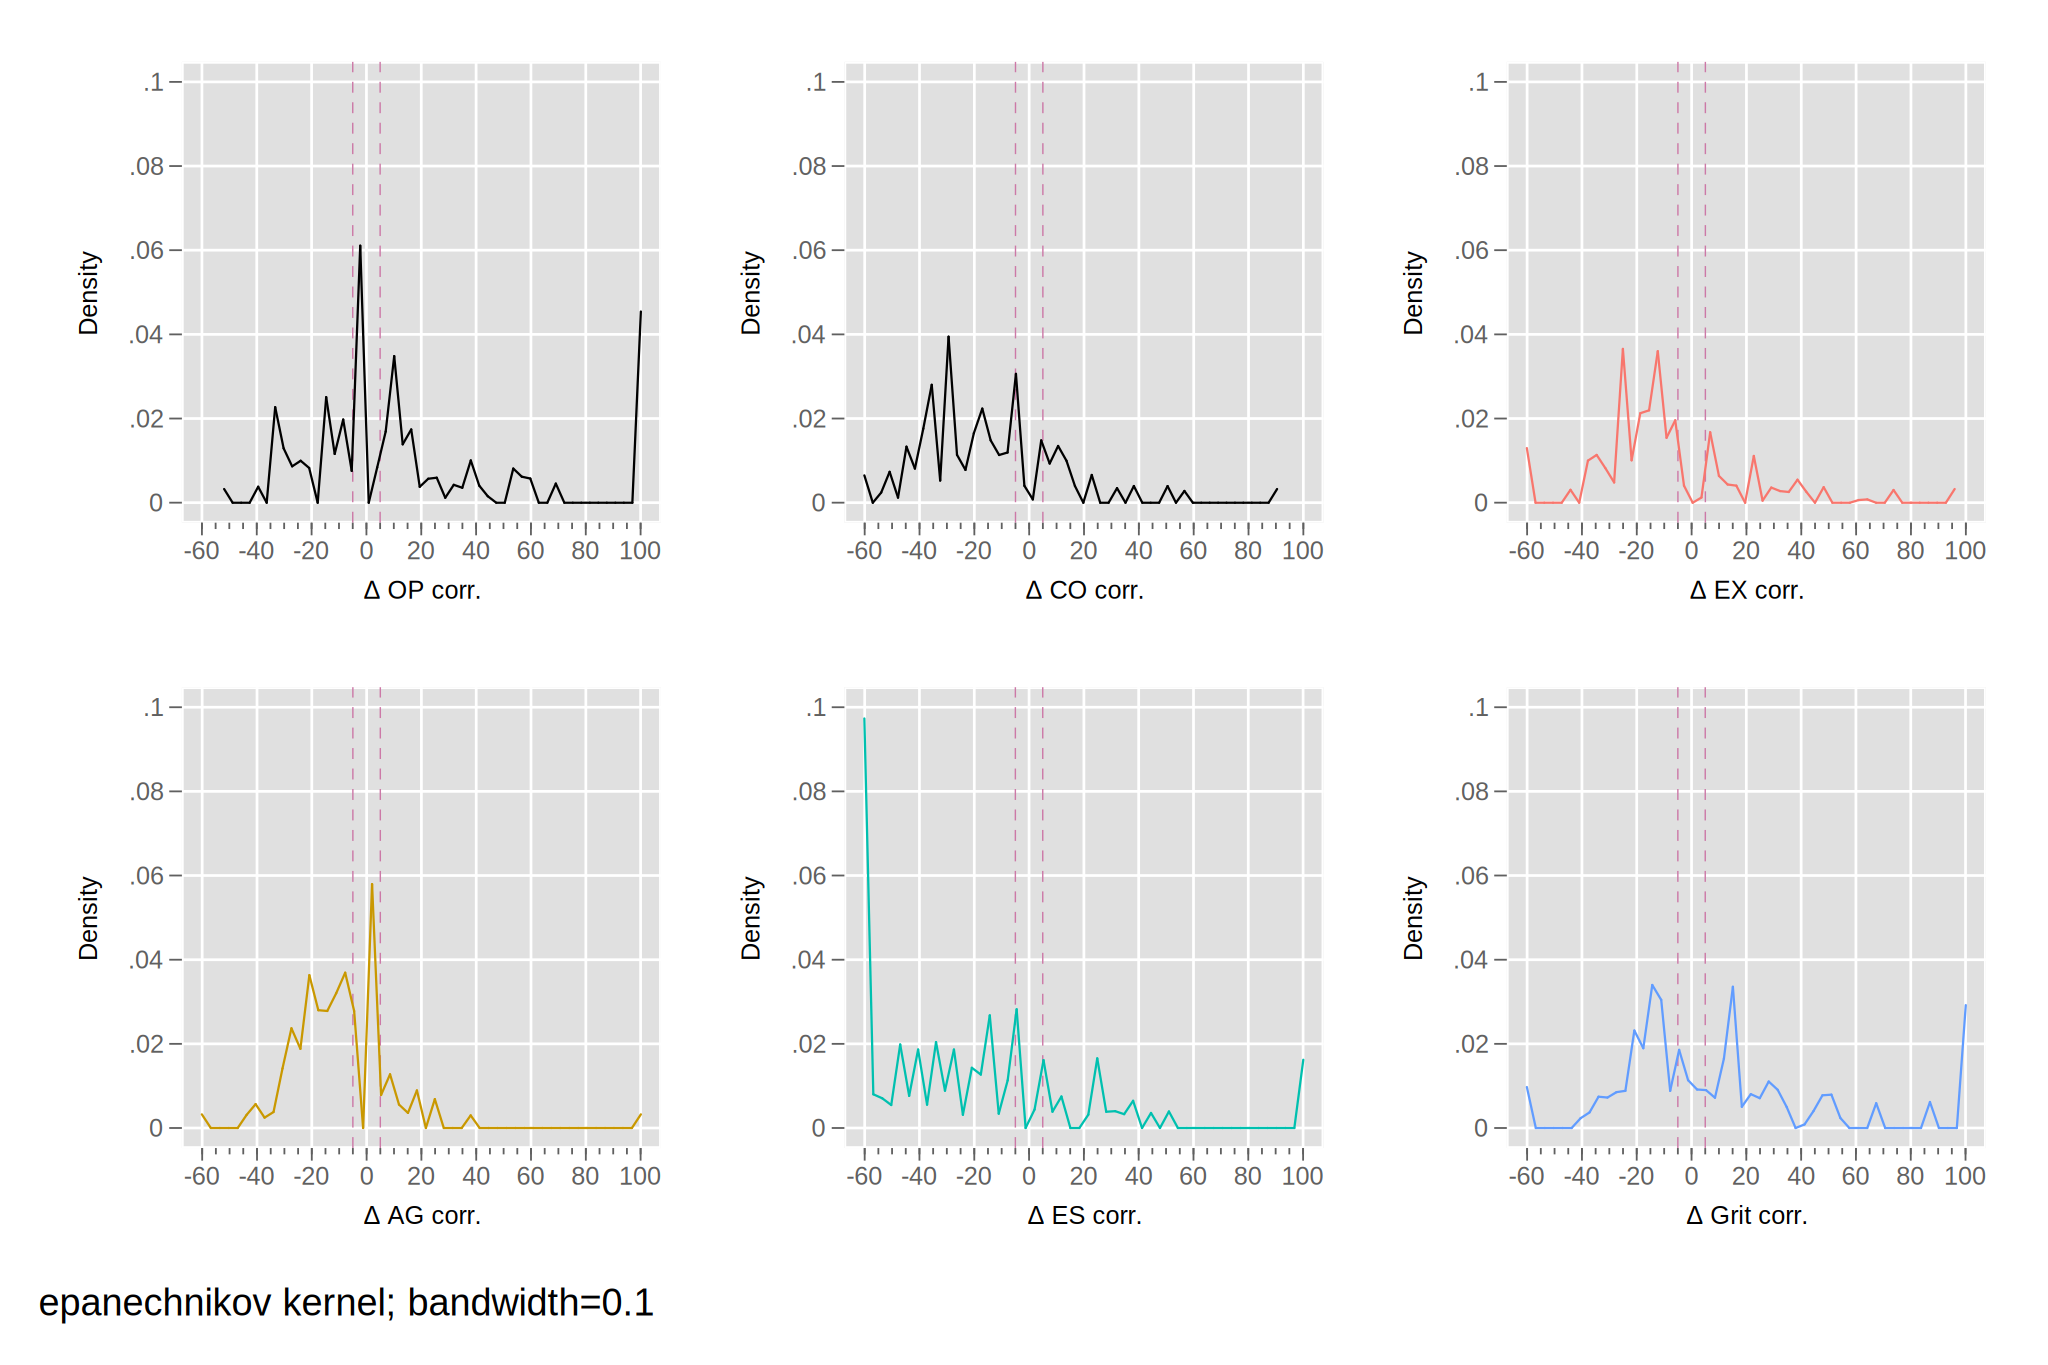
\includegraphics[width=\textwidth]{INPUT/Stabcorr}
\caption{Stability over time of Big-5 personality traits -- Distribution of variation rate between 2016-17 and 2020-21 for Big-5 personality traits corrected from acquiescence biais.}
\sourcefig{NEEMSIS-1 (2016-17) \& NEEMSIS-2 (2020-21); author's calculations.}
\label{fig:stab}
\end{figure}



\paragraph{Factor analysis}
As warned by \cite{Laajaj2019}, the Big-Five taxonomy is limited in developing countries for several reasons: the enumerator-respondent interactions (i) in face-to-face survey can induce a bias; the low education levels (ii) can make questions more difficult to understand and can induce a systematic response patterns, especially the acquiescence bias (iii).

The very good knownledge of the field allow us to collect data of high quality and avoid a bias due to misunderstanding of questions.
Moreover, we implement our own factor analysis of the 41 questions by principal component with promax rotation.
To avoid a bias in factor analysis, we do not corrected for acquiescence bias\footnote{La correction du biais d'acquiesence s'effectue sur la Big-5 taxonomy en regardant des questions censé être similaire. Or, elles sont similaires si l'on se base sur la Big-5 taxonomy et pour des WEIRD people. Dans un autre contexte ces questions peuvent avoir un sens tout à fait différent, d'où le fait que nous ne corrigeons pas. Nous ne voulons pas forcer un couple de question à être similaire.}.

The resulting factors are relatively similar to the Big-5 personality traits (see Table \ref{table:efa_corr} of Appendix \ref{section:efa_big5}) with satisfactory Cronbach's $\upalpha$:
\begin{itemize}
\item[Factor 1] as Extraversion-Openness ($\upalpha=0.89)$;
\item[Factor 2] as Conscientiousness ($\upalpha=0.87)$;
\item[Factor 3] as Emotional stability-Conscientiousness ($\upalpha=0.76)$;
\item[Factor 4] as Emotional stability ($\upalpha=0.75)$;
\item[Factor 5] as Agreeableness ($\upalpha=0.54)$.
\end{itemize}


\paragraph{Life-cycle effects}
To mitigate against the potential problem of life-cycle events\footnote{That might induce endogeneity with measurement error.}, we run univariate OLS regression (see equations i and ii below) with cognitive skills $S_k$ (where $k=1, 2, 3$ for raven, literacy, numeracy) and personality traits $P_k$ (where $k=1,...,10$ for Big-5 personality traits and factor analysis traits) as endogenous variables and age $A$ as exogenous variable.
We standardised the resulting residuals $\hat{\upvarepsilon_j}$ of equations $S_k=\upphi A+\upvarepsilon_j$ (eq. i) and $P_k=\upphi A+\upvarepsilon_j$ (eq. ii) and use it as cognitive and personality measures net of life cycle influences \citep{Nyhus2005, Brown2014}.




	% ******************************
	\subsection{Indebtedness measures}
	% ******************************

Before exploring the role of cognitive skills and personality traits, it is necessary to discuss debt and over-indebtedness measures.
There is no consensus in the literature but three approaches are often retained \citep{Betti2007, Ferreira2000}.
Objective measures focus on the ability (or inability) to service or repay debts.
Typically, it is the debt to income ratio, debt to asset ratio, debt service ratio.
Over-indebtedness occurs when a certain threshold is exceeded.
Although this is the most widely used measure, it under-estimate the burden of debt in ousting personal feeling and sacrifice associated with debt and over-indebtedness \citep{Betti2007}.
 
Subjectives measure assume that ``individual households are the best judges of their own net debt/wealth position'' \citep{Betti2007}.
The robustness of the results are based on the degree of honesty and literacy of individuals that can make it, sometimes, less reliable \citep{Betti2007, DAlessio2013}.
As stated by \cite{Rinaldi2006} and \cite{Keese2012}, in general, objective measures align quite well with subjective measures at the household classification level.

Administrative measures treat indebtedness and over-indebtedness as ``all cases
where non-payment of debts have been registered officially or declared before a court'' \citep{Betti2007}.
In rural Indian context, this type of measures have little meaning since most of the debt is informal.

In order to best measure the debt, we could combine objective and subjective measures as \cite{Aniola2012} do in European Countries, but this brings the risk that all households will find themselves categorized as over-indebted according to the measure used \citep{Chichaibelu2018}.

It is recommended to analyse indebtedness at household level because generally income is grouped between household members \citep{European2010}.
However, in order to explore the role of individual characteristics such as personality and cognitive skills on indebtedness, we focus on three types of individual objective measures allowing us to understand the debt from three angles.

First, to understand the role of personality traits \& cognitive skills on the incidence of individual debt and her extent, we use three dependents variable: the probability of being in debt\footnote{Dummy variable equal to 1 if the individual has some unsettled debt taken out in her own name, 0 otherwise.} in 2020-21; the number of loan taken by an individual and the total amount of individual debt\footnote{The sum of all unsettled debt taken out in her own name.}.

Second, we wish to understand the burden of debt in investigating the role of personality traits \& cognitive skills on the Individual Debt Service Ratio (IDSR\footnote{$IDSR=\frac{Individual~Debt~service}{Individual~Annual~Income}$ which represent the share of income required to cover the repayment of interest and principal on a debt for one year.}); on the Share of Household Debt held by the Individual (SHDI\footnote{$SHDI=\frac{Individual~Debt}{Household~Debt}$}); on the probability that an individual encountering problem during repayment of debt\footnote{} and on the probabilty of being over-indebted.
To measure over-indebtedness, we dichotomize IDSR at 0.3 and 0.4 threshold.
Thus, an individual is considered to be over-indebted when it is annual debt represent more than 30-40\% of his annual income \citep{Chichaibelu2017, DAlessio2013}.

Last, we analyse personality traits \& cognitive skills on the characteristics of debt through: the share of formal and informal debt on individual debt; the share of debt generating and not generating income on individual debt (see Table \ref{tab:usedebt} and \ref{tab:sourcedebt}) and the probabilty to pay interest.

%Despite the no conceptual consensus on what constitutes indebtedness and how it ought to be measured, DSR represents the most use ratio in the literature \citep{Chichaibelu2017, DAlessio2013}.






	% ******************************
	\subsection{Econometric framework}
	% ******************************

\paragraph{Selected sample}
In order to understand the relationship between personality traits \& cognitive skills in $t$ and indebtedness situation in $t+1$ in a constraint environement, we use split sample.
Even if statistical power is not maximal, it allow different effects of all independent variables between groups.

\paragraph{Data structure and clustering}
As mention earlier, in our data, individual questionnaire concerned two individuals ``egos'' of each household.
In analyzing debt at individual scale here, we investigate the role of personality traits \& cognitive skills for all ``egos''.
Question of the allocation of ressources within household is, obviously, essential in this configuration.
Indeed, \citep{Lazear1988}
\citep{Bonke2015} We find that in most households the income distribution is correlated with the sharing of consumption—the economic approach—and that this holds true even if the household pools its resources—the economic psychology approach, implying that there is no strong relationship between the two approaches.

Thus, we clustered error by households to take into account the fact that observations within each household are not independently and identically distributed.

As stated by \cite{Reboul2021} about intra-household cooperation over debt repayment:

% The fact that women are considerably more deeply indebted than men, and mostly to help make ends meet, obviously raises questions about how men assist financially, and more generally about intra-household cooperation. 
% Further research is needed on this critical issue. 
% While our data is limited, it suggests that fully pooling and sharing the household debt burden is not the norm.
% Whether debtors had assistance with repayments is only recorded in our data for a subsample of the loans: 52\% of the total in frequency. 
% Those were the loans that respondents highlighted as the most critical to repay, with a maximum of three per household.
% This subsample of ‘‘main loans” is therefore not representative; yet since their settlement is seen as critical, it seems quite probable that the potential bias would be towards overstating intra-household cooperation.
% As it turned out, debtors declared not to receive any help for the vast majority of the main loans (Table 5).
% While female main loans clearly more often benefit from help than male ones, female debtors still have to contend with two thirds (64\%) of their main loans on their own.
% Overall, these descriptive statistics suggest that while women and men seem to have a similar propensity to borrow, women get into debt far more heavily in relation to their incomes. 
% Furthermore, they predominantly and more frequently than men borrow for non-productive purposes, to smooth consumption and to ensure household reproduction. 
% They also more often put their loans towards repaying other loans.
% Microcredit clients, who are more deeply indebted, follow this pattern. 
% Last, women seem to have greater financial responsibilities in poorer and Dalit households, two categories that substantially overlap. 


\paragraph{Estimators}

We can classify our dependent variable sur leurs types (Table \ref{tab:recapY}).



\begin{table}[htbp]
\raggedright
\begin{tabular}{lcc}
\toprule
Variable & Type  & Estimator \\
\midrule
In debt (=1) & Dummy & Probit \\
Number of loans & Count & Poisson \\
Loan amount (1,000 INR) & Continuous & OLS \\
IDSR (\%)  & Proportion & OLS\sym{*} \\
SHDI  & Proportion & GLM \\
Problem to repay (=1) & Dummy & Probit \\
Over-indebted at 0.3 (=1) & Dummy & Probit \\
Over-indebted at 0.4 (=1) & Dummy & Probit \\
Share of formal debt & Proportion & GLM \\
Share of informal debt & Proportion & GLM \\
Share of income generating debt & Proportion & GLM \\
Share of non-income generating debt & Proportion & GLM \\
\bottomrule
\Tablenote{3}{\sym{*} 20\% of individual have a IDSR higher than 100\%, thus GLM with a \\ binomial distribution and a logit link function is not efficient (as for other \\ proportion variable).} \\
\end{tabular}%
\end{table}%


\begin{enumerate}%[leftmargin=*]
\item[i] Probit with ML estimation 

\begin{equation}\label{eq:probit}
\begin{split}
P(Y=1|x)=\upphi(\upbeta_{0}+X'_{1}\upbeta_{1})
\end{split}
\end{equation}


\item[ii] Poisson pour $\uplambda =$ parametre de la loi de Poisson 

\begin{equation}\label{eq:poisson}
\begin{split}
P(Y=y)=\frac{e^{-\uplambda}\uplambda^{y}}{y!}
\end{split}
\end{equation}


\item[iii] OLS 
Unlike \cite{Brown2014}, we do not use tobit model because the data are not censored, but defined on $\mathbb{R}^{+}$ \citep{Maddala1991}.

\begin{equation}\label{eq:ols}
\begin{split}
Y_{it}~=~\upalpha~+~X'_i\upbeta~+~Z'_{it}\upgamma~+~\overline{Z'}_{it}\uppi~+~\upepsilon_i
\end{split}
\end{equation}



\item[iv] GLM with a binomial distribution and a logit link function proposed by \cite{Papke1996}
The bounded nature of the dependent variable makes indeed a linear regression inappropriate (Cox, 1996; Papke \& Wooldridge, 2008),


\begin{equation}\label{eq:glm}
\begin{split}
Y_{it}~=~\upalpha~+~X'_i\upbeta~+~Z'_{it}\upgamma~+~\overline{Z'}_{it}\uppi~+~\upepsilon_i
\end{split}
\end{equation}



\end{enumerate}



\paragraph{Control variables}
Dire que ca aussi c'est en t, il y a que la dette qui est en t+1

Our control variables are based on \cite{Reboul2020, Brown2014, Chichaibelu2017} which take the existing classic controls. 
We use two vector of variables.

$C'_{indiv,i}$ for individual level variables includes: age; age square; dummy variable which take 1 if individual is the household head, 0 otherwise; main occupation\footnote{Define as the most time-consuming activity.}; number of occupation (dummyvariable if plusieurs occupations plutôt); dummy variable which take 1 if individual received formal education through school, 0 otherwise (no formal education) and a dummy variable for marital status (1 if married, 0 otherwise). 
And households controls: 

$C'_{HH,i}$ for household level variables: monetary value of assets\footnote{The monetary value of assets includes the monetary value of gold; land; house; livestock; agricultural equipment and consumption good such as car, computer, cookgas, phone, etc.}; sex ratio; annual income; household size; number of children (individual under 16 years old); shock exposure (dummy variable which take 1 if the household experienced a shock\footnote{Marriage of at least one of the household members or/and household surveyed after the demonetisation.} between 2010 and 2016-17, 0 if not); number of income sources. 





%\paragraph{Caveat}
%An important caveat to acknowledge is the fact that this paper does not claim to seek causality. 
%Although we assume that personality traits are exogenous regressor, there is no consensus among psychologist as we note earlier.
%As many other paper \citep{Brown2014, Bucciol2017, Pinjisakikool2017, Pinjisakikool2017b, CobbClark2016, Bertoni2019}, our empirical analysis relate to correlation because of we cannot rule out the possibility of reverse causality between our endogenous variables and our supposed exogenous personality traits.
%At the time of writing, only \cite{Parise2019} deal with reverse causality issue in instrumenting conscientiousness and neuroticism with exposition to shock during childhood.




\newpage
% ***********************************
\section{Descriptive statistics}
% ***********************************




%\cite{John1999} the Big 5 "represent personality at the broadest level of abstraction, and each dimension summarizes a large number of distinct, more specific personality characteristics".

\begin{figure}[ht]
\raggedright
\includegraphics[width=\textwidth]{INPUT/Kernel_perso}
\caption{Distribution of cognitive skills and personality traits -- The resulting cognitive score and personality trait is based on the standardised residual from univariate OLS regression with age as exogenous variable. This is the cognitive score and personality trait purged from life-cycle effects}
\sourcefig{NEEMSIS (2016-17); author's calculations.}
\label{figure:EGOscore}
\end{figure}





	% ***********************************
	\subsection{Descriptive analysis}
	% ***********************************

		% ***********************************
		\subsubsection{Study population}
		% ***********************************
		
%\subimport{INPUT}{table_HHcharact.tex}


On average, we find between 4 and 5 individuals per household [and between 1 and 2 childrens per household] in 2010 and 2016-17 and we do not note any significant difference between caste group [except for the upper caste who have on average less than one children per household].
Whatever the caste, for almost half of households, men outnumber women. 




		% ***********************************
		\subsubsection{Who is ego?}
		% ***********************************
		
%\input{INPUT/table_EGOcharact.tex}


The majority of men are the head of household.% and this share increased between 2010 and 2016-17 because of for some households, the head in 2016-17 is the son in 2010 (other cat.).
%The same observation is true for women: the wife in 2010 become the mother of 2016-17.
Despite the small share, it is important to note that more than 20\% of women are the head of household in our sample.
Finally, womens are more enrolled in non stable activity as casual agriculture and NREGA programs (Other) than men.
Indeed, most men get the majority of their income from self-employement agriculture, non-agricol regular work or self-employement.


Concerning the cognitive skills, on figure \ref{figure:EGOscore} we observe several differences between men and women insofar as men have higher score than women for the three measures.
%It is also the men who are more educated so we can easily say that is the effect of school (vérifier la littérature dessus car si ca se trouve ce n'est pas du tout le cas).
\dev{Changer, dire que c'est avec l'analyse factorielle et changer tous les commentaires du coup.} For the Big-Five personality traits note several differences between men and women in terms of score.
For extraversion where the distribution of men are more oblique to the right, which means that they have higher extraversion score.
This is the inverse for women for conscientiousness: the distribution is oblique to the left compared to men, which means that they have lower conscientiousness score.
For the emotional stability, the distribution is more leptokurtique for women than for men, which means that the men are more evenly distributed in terms of score than women.
Finally, we do not note differences in terms of openness and agreeableness between men and women.

		% ***********************************
		\subsubsection{Indebtedness trend}
		% ***********************************






\newpage
% ***********************************
\section{Results}
% ***********************************

%https://www.jwe.cc/2012/03/stata-latex-tables-estout/
% \begin{table}[htpb]
% \centering
% \begin{threeparttable}
% \caption{Total sample and first part of main variables}
% \label{econ:all_global_p1}
% \estauto{INPUT/econ_all_global_p1}{8}{S S S S S S S S}
% %\starnote
% \fignote{$\sym{*}~~p<0.10, \sym{**}~~~p<0.05, \sym{***}~~~~~p<0.01$. $\ssymbol{2}$ for 1,000 INR. $\ssymbol{3}$ Owner.}
% \sourcetab{RUME (2010) and NEEMSIS (2016-17); author's calculations.}
% \end{threeparttable}
% \end{table}	






\newpage
% ***********************************
\section{Conclusion}
% ***********************************

% 

\clearpage
\newpage
%-------------------------------------------------------------------------------%
%\begin{nolinenumbers}
\addcontentsline{toc}{section}{Références}
\bibliography{C:/Users/Arnaud/Dropbox/Arnaud/Ref_Arnaud}
%\nocite{*}



\newpage
%-------------------------------------------------------------------------------%
\appendix

\section{Data description}

\input{INPUT/appendixcaste}

\section{Factor analysis for personality traits}
\label{section:efa_big5}

%\input{INPUT/big5classification}

\input{INPUT/factor1}
\input{INPUT/factor2}
\input{INPUT/factor3}
\input{INPUT/factor4}
\input{INPUT/factor5}
\input{INPUT/factor_std}
\input{INPUT/big5_factor_corr}

% Table generated by Excel2LaTeX from sheet 'descX1'
\begin{table}[htbp]
  \raggedright
  \caption{One-way ANOVA for personality traits and cognitive skills}
    \begin{tabular}{lcccccccc}
    \toprule
    Source & SS & df & MS & F-stat & p-value &       & $\upchi^2$$\ssymbol{1}$  & p-value \\
    \midrule


    \bottomrule
	\Tablenote{9}{$\ssymbol{1}$ Bartlett's test. Although there is much debate, we admit that when the sample \\ size is similar, ANOVA is robust to difference in variance between groups \citep{Box1954}.} \\	
    \end{tabular}%
  \label{tab:anovaperso}%
  \sourcetab{NEEMSIS-1 (2016-17); author's calculations.}
\end{table}%






\clearpage
\newpage
%-------------------------------------------------------------------------------%
\setcounter{tocdepth}5
\tableofcontents

%\end{nolinenumbers}
\end{document}


% % ***********************************
% \subsection{Hypothesis}
% % ***********************************

% As we already note, the goal of this paper is to analyze the role of cognitive skills and personality traits on indebtedness in a context where \jati and gender conditionned individuals.


% firstly, check the contextual determinants of debt.
% Then, we add personality traits \& cognitive skills in the analysis to answer our first question: is cognitive skills and personality traits plays a significant role on indebtedness situation of households in rural India?
% Following literature, we can make H\ref{hyp:stability}.
% Indeed, concerning conscientiousness, \cite{Donnelly2012} state that ``highly conscientious individuals manage their money more because they have positive financial attitudes as well as a future orientation''.
% \cite{Brown2014, Nyhus2001} find similar results: conscientious individuals are less likely to have ever been in debt and conscientiousness is negatively related to the amount of unsecured debt.
% \cite{Nga2013} find that conscientiousness have a significant influence on risk aversion in Malaysia.
% \cite{Forlicz2019} find that for most of these countries there existed significant differences between debtors and debt-free individuals regarding the level of conscientiousness
% For neuroticism, \cite{Pinjisakikool2017b} find that emotional stability (inverse of neuroticism) significantly predict financial risk tolerance.

% \begin{hyp}[H\ref{hyp:stability}] \label{hyp:stability}
% Conscientiousness and neuroticism play significant role on household indebtedness [and over-indebtedness].
% \end{hyp}

% To understand the phenomenon more in depth, we decompose the analysis by caste, class and gender.
% The notion of class allow us to encompass ``property, wealth, occupation, income, and education'' \citep{Beteille2007}.
% We implement a multiple correspondance analysis with land property, wealth, occupation and income\footnote{We choose to not take into account education to stay at household level.} to create a dichotomy between high and low class (see appendix \ref{section:mca_class}).
% For caste and class decomposition, we formulate H\ref{hyp:poorer} imagining that cognitive skills are more important for lower households because we can imagine that higher one have all a high level of cognitive skills (math, literacy, etc.) because of better level of education\footnote{For the link between caste and education, see \cite{Borooah2005}.}.
% %\cite{Gaurav2012} find that cognitive skills significantly predict the financial aptitude and debt literacy for rural farmer in Gujarat
% %\cite{Agarwal2013} finds that ``consumers with higher math scores, are substantially less likely to make a financial mistake'' in separating our sample between economically and socially upper households and economically and socially lower households.
% \begin{hyp}[H\ref{hyp:poorer}] \label{hyp:poorer}
% Cognitive skills are better predictors for lower households than for higher one. 
% \end{hyp}

% Concerning gender, as \cite{Reboul2020} stated: ``[w]omen in the poorest households, despite meager incomes, have the highest borrowing responsibilities, shouldering the highest shares of household debt. [...] Their larger role in household debt management may be linked to their greater mobility and lower restrictions on social interactions, notably with men, which would underpin both their greater income shares and their access to credit relations. ''
% Thus, we can formulate the H\ref{hyp:women} hypothesis.
% \begin{hyp}[H\ref{hyp:women}] \label{hyp:women}
% When ego is a woman, her cognitive skills and personality traits play a bigger role in household finances than when ego is a man.
% \end{hyp}

% \cite{Reboul2019} Far beyond the issue of information about wages, the management of family finances leads
% to constant tensions and conflicts among family members, and thus gives rise to various tactics
% aimed at partially overcoming family constraints. This is particularly true for women, who have
% a heavy responsibility to ensure, among other things, daily expenses


% Last, we explore the source and use of debt in creating the dichotomy formal--informal and income generator--non-income generator of debt.
% Following results of \cite{Brown2014}, we formulate H\ref{hyp:filr}.
% \begin{hyp}[H\ref{hyp:filr}] \label{hyp:filr}
% Conscientiousness, extraversion, agreeableness and openess to experience have an association with informal debt.
% \end{hyp}

% To try to verify our hypotheses, we use original data set from rural south India.

% \cite{Guerin2014a} il faut aussi que je regarde le rôle des compétences cognitives sur la négociation de la dette en cross section : qui sont ceux qui arrivent le mieux à négocier leur dette ? 
% Comment savoir la negociation de la dette ? C'est le prix de la dette
% Prix de la dette p16 de \cite{Guerin2014a} The cost of \textit{terinjavanga} loans








% % ***********************************
% \section{Pistes en réflexions}
% % ***********************************

% \begin{itemize}[label=--]
% \item Quel est le score de l'\textit{homo oeconomicus} en termes de \textit{Big Five} ? \citep{Lopez2020}
% \item À partir de là, on peut chercher à voir si les autoentrepreneurs sont des \textit{homo oeconomicus} ou s'ils sont \textit{schumpeterien} ou \textit{coasien}.
% \item Analyse \textit{schumpeterienne} : \url{https://doi.org/10.4000/interventionseconomiques.1481}
% \item Regarder les articles de \cite{Gong2020} et de \cite{Srinivasan2005}
% \item Voir Occupational Attainment and Earnings in Southeast Asia: The Role of Non-cognitive Skills de Labour Economics, 2020
% \item salaire (y) = perso (x) -> OK; salaire (y) = perso (x) + educ (x) -> pas OK; perso passe par educ
% \item soulèvent; pointent; surlignent; mettent en évidence
% \item \cite{Yilmazer2005} + \cite{Poterba2001} + \cite{King1982}
% \end{itemize}





%---------------------------------
%KEEP THAT BUT NOT IN THE ARTICLE
%---------------------------------
%\paragraph{Retirement assets}
%Compared to China, the retirement pensions are not very efficient.
%Indeed, around 90\% of labor is informal [in the sense of absence of social insurance] and 85\% of non-agricultural workforce is informal \citep{Mehrotra2019}.
%For \cite{Badarinza2016b}, India figures as an outlier among low-middle-income countries on this point.
%\paragraph{Gold}
%\begin{itemize}
%\item On average, gold represent more than 11\% of indien household balance sheet  while it is less than 1\% in China \citep{Badarinza2016b}.
%\item Préciser les différences rurales urbaines de \cite{Badarinza2016b}.
%\item Mais rester sur le fait qu'au TN l'or est la première forme d'épargne d'après \cite{Roesch2008} \cite{Guerin2012a}
%\item Pourquoi ils aiment tant ?
%\item[1] Real estate has lower liquidity when compared with gold, and if liquidity needs are correlated with inflation volatility, gold better serves the purpose than real estate. Gold as a non-financial asset also has additional properties that are not provided for by real estate, such as a high collateral value and physical verifiability \citep{Badarinza2016b}
%\item[2] Avec la littérature d'Isabelle, parler du social role de l'or en rural India.
%\end{itemize}
%---------------------------------






% Mesure overindebtedness
% \item \citep{European2010} ont 5 recommendations pour bien mesurer:
% \item[1] Le surendettement s’analyse au niveau du ménage car les revenus des individus sont généralement regroupés ;
% \item[2] Les indicateurs doivent couvrir tous les aspects des engagements financiers : le logement, le crédit à la consommation, les factures, les emprunts hypothécaires ;
% \item[3] Le surendettement est considéré comme un état structurel car il implique une incapacité à faire face à des dépenses récurrentes ;
% \item[4] Le surendettement ne se résout pas en empruntant davantage ;
% \item[5] Pour qu’un ménage respecte ses engagements, il doit réduire considérablement ses dépenses ou trouver un moyen d’accroître ses revenus.

